\section{Estensioni e originalità}
\label{cap:extensions-and-originalities}

Oltre alle 3 implementazioni richieste dalla consegna dell'homework, abbiamo deciso di esplorare qualche altra estensione degli algoritmi per il calcolo del Minimum Spanning Tree visti a lezione.

\subsection{Prim con k-ary Heap}

% ...

Dal punto di vista teorico, le Fibonacci Heap hanno una complessità temporale migliore delle k-ary Heap.
Tuttavia, dal punto di vista pratico, le k-ary Heap hanno una performance migliore perché la loro struttura permette loro di sfruttare la cache locality. Inoltre le Fibonacci Heap hanno un coefficiente di complessità nascosto piuttosto elevato.
Un altro motivo per cui abbiamo deciso di non implementare le Fibonacci Heap è che sono più complesse da implementare rispetto alle k-ary Heap. \\

\noindent Quando le k-ary heap sono usate per implementare code di priorità, l'operazione di aggiornamento del valore della chiave è più veloce rispetto ad una Binary Heap (\complexityLogN{} per le Binary Heap contro \complexityLogkN{} per le k-ary Heap).
L'operazione di rimozione dell'elemento con minore chiave, tuttavia, aumenta a \complexityKLogkN{} rispetto a \complexityLogkN{} delle Binary Heap. Ma visto che nell'algoritmo di Prim le operazioni di cambio valore delle chiavi sono più comuni delle operazioni di estrazioni del minimo elemento, le k-ary Heap sono comunque più efficienti delle Binary Heap per quell'algoritmo.
% ...

\noindent Le figure \ref{fig:Prim2vsPrim4-500}, \ref{fig:Prim2vsPrim4-500} e \ref{fig:Prim2vsPrim4-80k-100k} mostrano una comparativa tra le performance
dell'algoritmo con una binary heap e un k-ary heap con $k = 4$. 
Da \ref{fig:Prim2vsPrim4-500} e \ref{fig:Prim2vsPrim4-2k-4k} si nota un lieve miglioramento delle performance utilizzando il k-ary heap, anche 
se questo comporta più uscillazione tra i tempi di runtime rispetto a input differenti. La figura \ref{fig:Prim2vsPrim4-80k-100k} invece mostra
una controtendenza tale per cui su input molto grandi il binary heap tende a fare lievemente meglio del k-ary heap.

\begin{figure}[H]
    \centering
    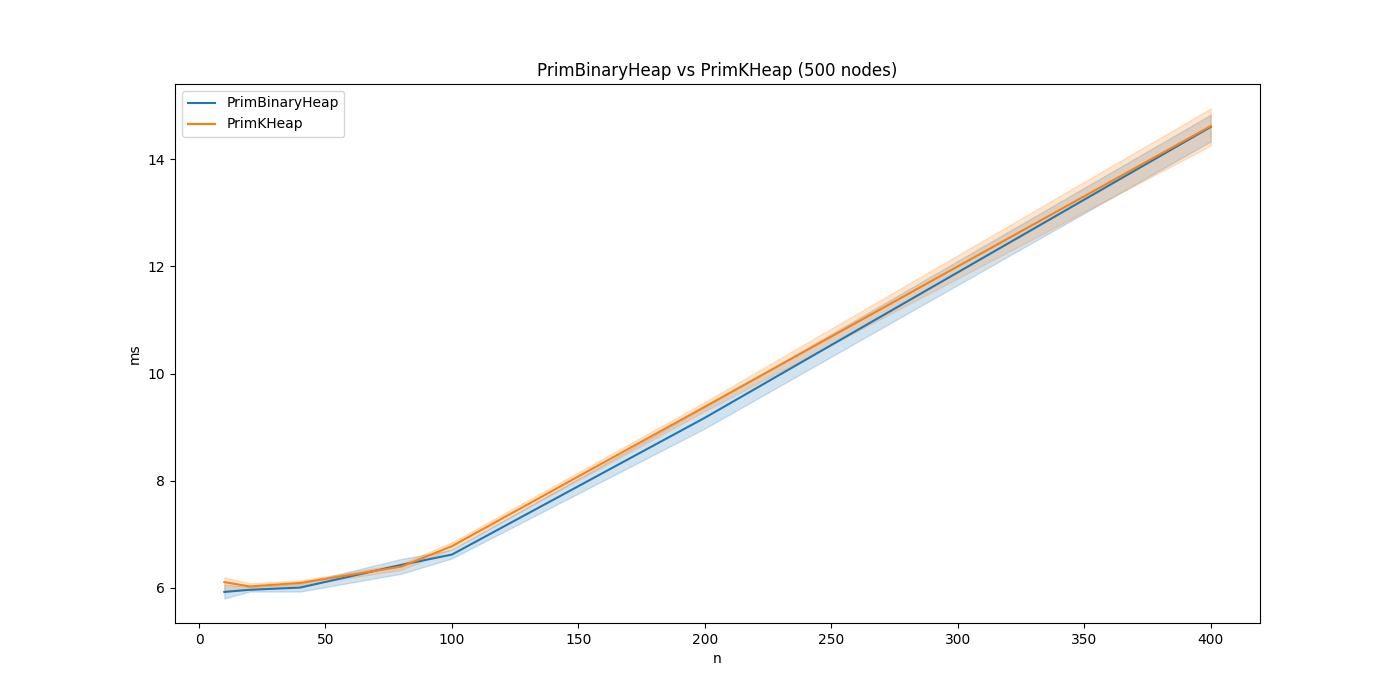
\includegraphics[width=1.0\textwidth]{./images/PrimBinaryHeap_vs_PrimKHeap_(500_nodes).png}
	\caption{Andamento di PrimBinaryHeap e PrimKaryHeap con taglia dell'input da 0 a 500 nodi.}
    \label{fig:Prim2vsPrim4-500}
\end{figure}

\begin{figure}[H]
    \centering
    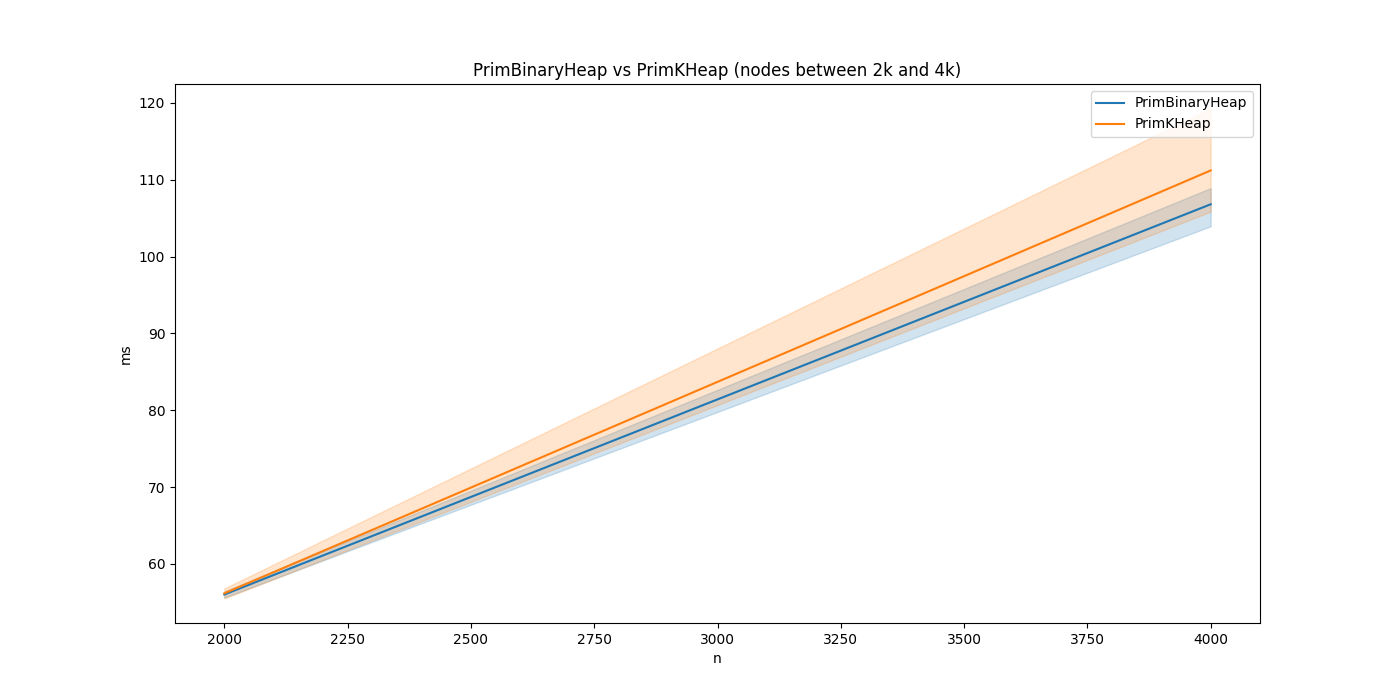
\includegraphics[width=1.0\textwidth]{./images/PrimBinaryHeap_vs_PrimKHeap_(nodes_between_2k_and_4k).png}
	\caption{Andamento di PrimBinaryHeap e PrimKaryHeap con taglia dell'input da 2k a 4k nodi.}
    \label{fig:Prim2vsPrim4-500}
\end{figure}

\begin{figure}[H]
    \centering
    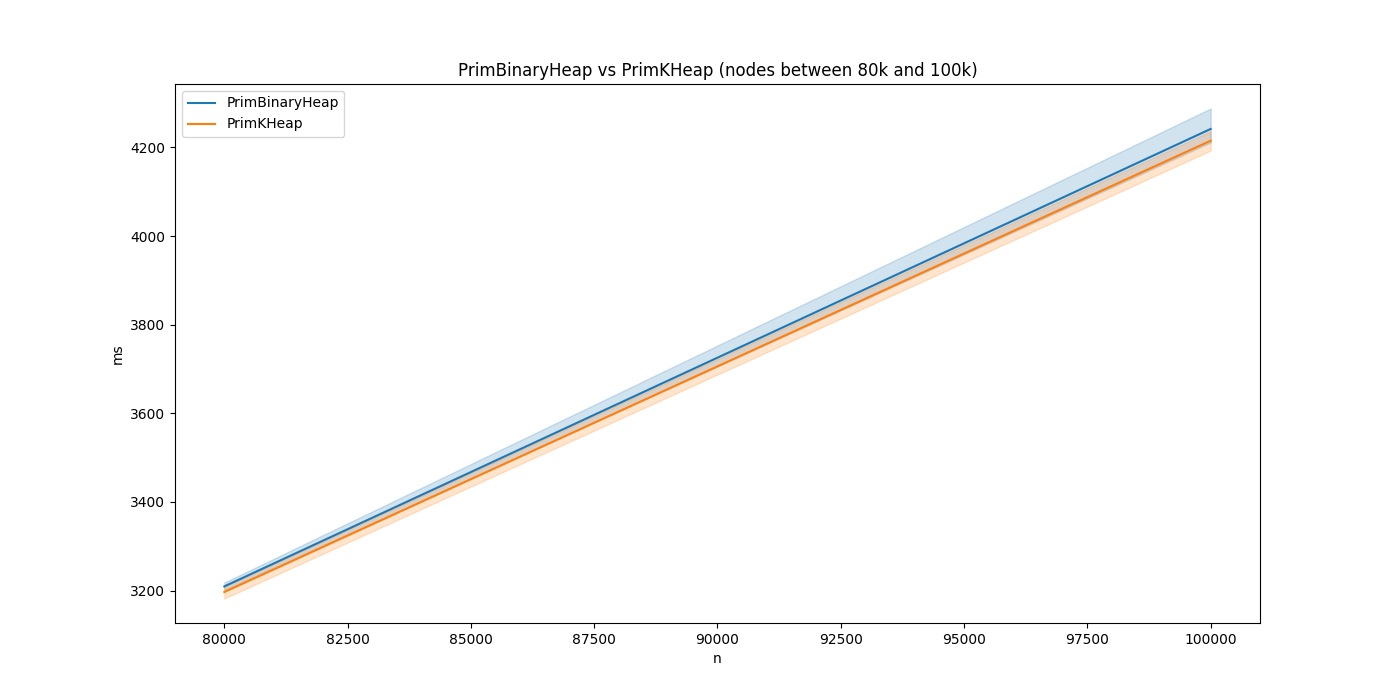
\includegraphics[width=1.0\textwidth]{./images/PrimBinaryHeap_vs_PrimKHeap_(nodes_between_80k_and_100k).png}
	\caption{Andamento di PrimBinaryHeap e PrimKaryHeap con taglia dell'input da 80k a 100k nodi.}
    \label{fig:Prim2vsPrim4-80k-100k}
\end{figure}

\subsection{Kruskal con Disjoint-Set e path-compression}

% path-compression via path-halving + union by size
